\section{Mobile devices and their evolution}
Today, the mobile devices' panorama is dominated by smartphones and tablets. Before the introduction of such devices, the market was very different, with the predecessors of the smartphones: PDAs.

\subsection{From PDAs to smartphones}
A \textbf{Personal digital assistant} (PDAs) is a mobile device that acts as a personal information manager. These type of devices were the \textbf{first attempt at providing the capabilities of a computer in a relatively small mobile device} (hence they were also known as handheld PC). A PDA device typically features:
\begin{itemize}
    \item \textbf{A display} (and possibly physical buttons, depending on if the specific model uses a touch display);
    \item \textbf{Audio capabilities} (with the possibility of using it as a portable media player);
    \item \textbf{Telephony} (acting as a mobile phone);
    \item \textbf{Internet connectivity} (only via Wi-Fi);
    \item \textbf{A web browser};
    \item \textbf{Bluetooth connectivity}.
\end{itemize}

In 1984 Psion released the first PDA: the Organiser I; the term PDA though came to existence in 1992, once Apple released the Apple Newton. PDAs started to include telephony capabilities in 1994 with the IBM Simon; this device is particularly important, since it can be considered the first smartphone.
\vspace{5mm}

\begin{figure}[!ht]
    \centering
    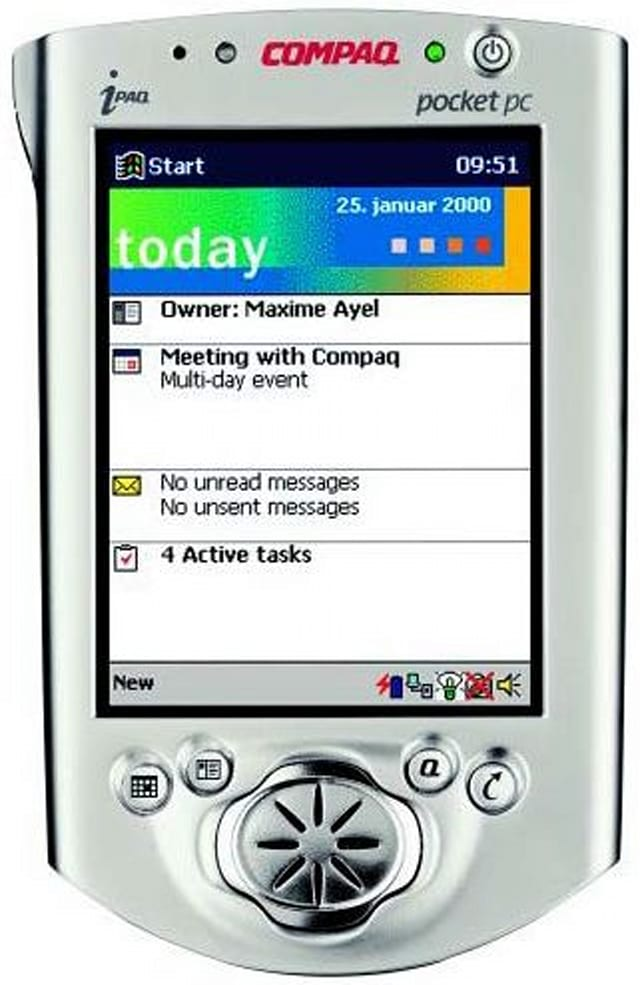
\includegraphics[scale=0.3]{document/chapters/chapter_1/images/compaq_ipaq_3650.jpg}
    \caption{Example of PDA device - Compaq iPAQ 3650}
    \label{fig:compaq_ipaq_3650}
\end{figure}

Although PDAs had a considerable share of the mobile market (but still dominated by traditional mobile phones), \textbf{in the mid-2000s PDAs started to be replaced more and more with modern smartphones} until they completely replaced them.
Today the term "personal digital assistant" has found a new meaning in the definition of virtual assistants based on speech synthesis (ex: Amazon's Alexa).

Contemporary mobile devices' market is not remotely comparable to the market of the PDAs era, reaching an \textbf{exponentially greater number of smartphones and tablets units sold}. Despite this, some experts think that the market is saturated, and it is reaching its peak \cite{smartphones_sales}. One important aspect of today's market is the fact that \textbf{the number of smartphones currently sold is far greater than the number of PCs sold} (that is actually gradually declining) as shown in \textit{figure \ref{fig:global_sales_of_pcs_and_smartphones}}.

\begin{figure}[!ht]
    \centering
    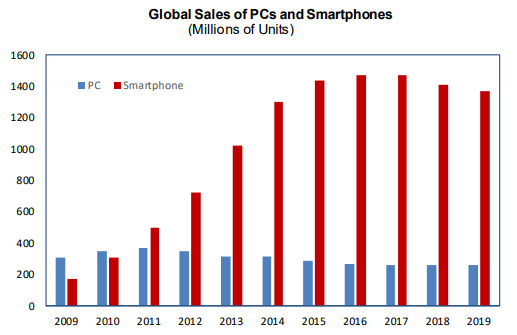
\includegraphics[scale=0.9]{document/chapters/chapter_1/images/global_sales_of_pcs_and_smartphones.png}
    \caption{Global Sales of PCs and Smartphones from 2009 to 2019 \cite{smartphones_sales}}
    \label{fig:global_sales_of_pcs_and_smartphones}
\end{figure}

\subsection{Technological progress}\label{technological_progress}
\textbf{Hardware has had a general improvement} in the computational world and mobile devices' technological capabilities are no exception; as can be seen in \textit{figure \ref{fig:pda_capabilities}}, PDAs had very poor performances able to only mildly satisfy the limited use cases of such devices. 

\begin{figure}[!ht]
    \centering
    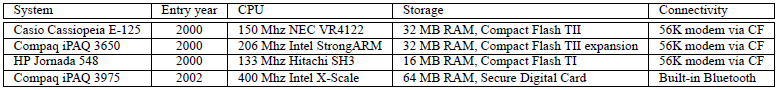
\includegraphics[scale=0.77]{document/chapters/chapter_1/images/pda_capabilities.png}
    \caption{Example of technological capabilities of 2000s PDAs \cite{integrating_mobile_devices_into_grid}}
    \label{fig:pda_capabilities}
\end{figure}

To better understand the \textbf{technological gap between devices from the year 2000 and today's smartphones}, {figure \ref{fig:three_systems_comparison}} provides a comparison between these three examples:
\begin{itemize}
    \item Compaq iPAQ 3650 (\textit{figure \ref{fig:compaq_ipaq_3650}}), the best PDA from \textit{figure \ref{fig:pda_capabilities}} among the ones that could also be connected to the internet;
    \item Power Mac G4 - M5184 (EMC 1864), the best possible configuration in the Power Mac G4 line from the year 2000;
    \item Xiaomi Redmi Note 9 Pro, a 2020 mid-range (as far as value for money) smartphone.
\end{itemize}
\vspace*{5mm}

\begin{figure}[!ht]
    \centering
    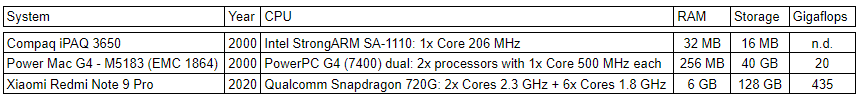
\includegraphics[scale=0.88]{document/chapters/chapter_1/images/three_systems_comparison.png}
    \caption{Comparing a 2020 mid-range smartphone to devices from the year 2000}
    \label{fig:three_systems_comparison}
\end{figure}

Despite information about the number of Gigaflops (billion floating point operations per second) for the Compaq iPAQ 3650 is not available anywhere, it can be confidently said that its value is far less than the 20 Gigaflops that the Power Mac G4's CPU was capable of; considering that the Redmi Note 9 Pro is capable of executing a number of floating point operations per second that is 21.75 times higher than the Power Mac G4, a modern smartphone outmatches a PDA by an enormous factor. Available RAM and Storage have also made a significant step forward, with the chosen smartphone having 187.5 times more RAM than the PDA and 8000 times more memory available for the storage. The gap has also to take into consideration other technologies of modern smartphones, such as Wi-Fi and 4G connections as a standard (with newer models moving towards 5G connections) and a multitude of sensors, as well as high resolution cameras. 
It is apparent that \textbf{modern smartphones are on a vastly different technological level compared to old PDAs, significantly outmatching also computers that coexisted with them}.
